%!TEX root = ../deco_star.tex

%-------------------------------------------------------------------------
\section{Design Features}\label{sec:design}
In regard to design features, on the one hand, creative pattern generation includes repetitive and ordered structures that are often considered as \textit{textures}, thus demanding automatic and procedural creation. On the other hand, creative pattern generation might also include a global layout, adapting to the space they are filling. Furthermore, this type of patterns might include visual hierarchies and highlights that are singularly placed with creative intent. 

Specifically, we categorize the analysis of the state of the art in \Cref{sec:analysis} with the design features \rev{Condensed layout:}{of \textit{Distribution and Repetition}, \textit{Frames and Hierarchies}, \textit{Curves, Lines and Brushing}, \textit{Connections, Branches and Directionality}, and \textit{Single Accents} for creative pattern generation. In the following we briefly explain each design feature and give a visual example for it from the related work.}

% TODO: replace all images with high-res version for submission

\rev{}{
    \noindent\textbf{Distribution and Repetition}

    Repetition and an overall distribution of elements usually result in homogeneous pattern with a texture-like quality. A careful composition of the repeating elements can be used to create a perception of balance and order. Compositions are not limited to the repetition of the same element, but different visual qualities such as size or saturation can create various relationships.
    \begin{figure}[H]
        \centering
            \revimage{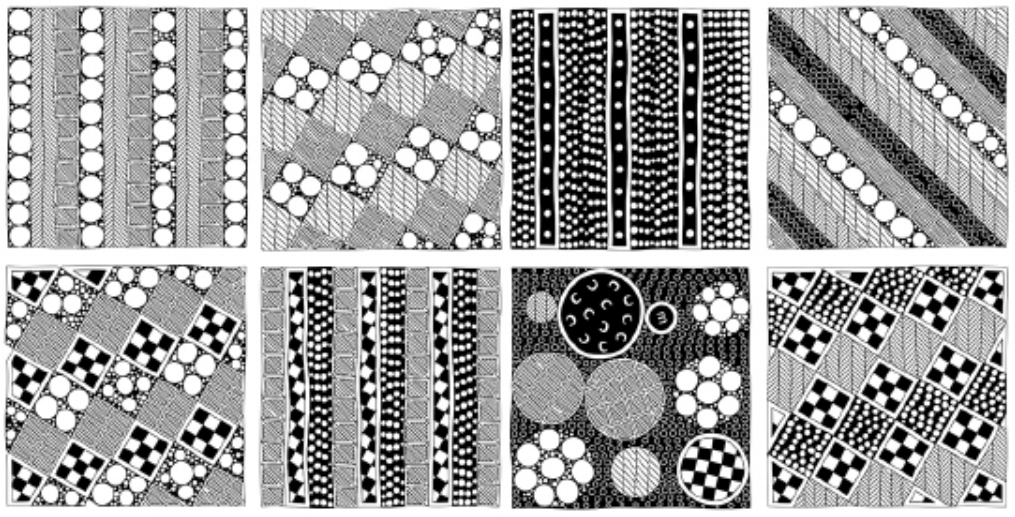
\includegraphics[width=\linewidth]{figures/design_features/santoni_2016_ggp.png}}
        \caption{Designs showcasing distribution and repetition as creation feature, leading to balanced as well as more irregular repetitive pattern designs. Example results from~\cite{santoni_2016_ggp} (Figure 10), \color{red}{Status rights: not started.}}
    \end{figure}
}

\rev{}{
    \noindent\textbf{Frames and Hierarchies}

    Frames and hierarchical compositions further structure a design by creating contrasts (e.g., foreground vs. background) and accentuating spatial relationships (e.g., framing). 

    \begin{figure}[H]
        \centering
            \revimage{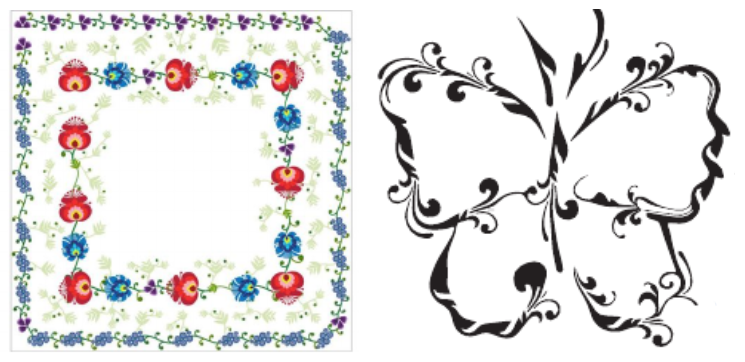
\includegraphics[width=\linewidth]{figures/design_features/frames_hierachies.png}}
            \label{fig:frames_hierachies}
        \caption{Designs using frames and a hierarchy of elements for structuring the space and/or a sense of foreground and background. Left, example result from~\cite{gieseke_2017_ooo} (Figure 7), right,~\cite{lu_2014_dds} (Figure 19). \color{red}{Status rights: not started.}}
    \end{figure}
}

\rev{}{
    \noindent\textbf{Curves, Lines and Brushing}

    Artist-defined curved elements and lines are an essential design feature for many creative pattern designs. They can be used, e.g., as base element or frame as well as distinct visual element. The technique of brushing usually gives a individual, hand-made quality to a pattern.

    \begin{figure}[H]
        \centering
            \revimage{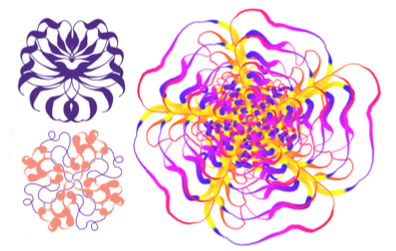
\includegraphics[width=\linewidth]{figures/design_features/jacobs_2018_dbe.png}}
        \caption{Designs using brushed curves as constituent design feature. Example result from~\cite{jacobs_2018_dbe} (Figure 1). \color{red}{Status rights: not started.}}
    \end{figure}
}


\rev{}{
    \noindent\textbf{Connections, Branches and Directionality}
    Connections and branches between base elements are often used to create frames and hierachies, as~\Cref{fig:frames_hierachies} shows. These structures and directionality are also often used to elaborate and accentuate the form of the space they fill, e.g. by aligning to it, building an pattern-object relationship \cite{arbruzzo_2006_dec}. 

    \begin{figure}[H]
        \centering
            \revimage{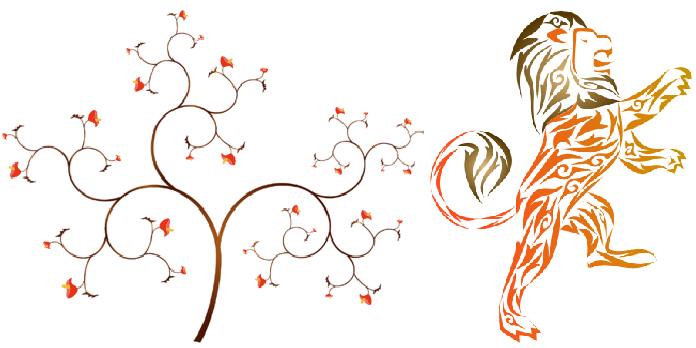
\includegraphics[width=\linewidth]{figures/design_features/branching_directionality.png}}
        \caption{Designs using branching and directionality, aligning elements to the shape they fill. Left, example result from~\cite{guo_2020_ipm} (Figure 1), right,~\cite{saputra_2017_ffo} (Figure 1). \color{red}{Status rights: not started.}}
    \end{figure}
}

\rev{}{
    \noindent\textbf{Single Accents}

    Single, visually dominant elements and structures might not follow the underlying order of a pattern, breaking an otherwise homogeneous appearance. This design feature is based on the principle of contrasts and accents, which are crucial for overall visual appeal of a creative pattern design~\cite{wong_1998_cgf,ward_1896_tpo, moughtin_1999_udo}.

    \begin{figure}[H]
        \centering
            \revimage{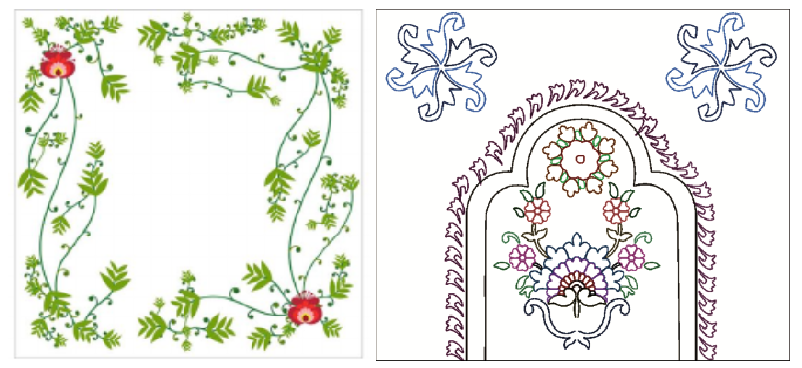
\includegraphics[width=\linewidth]{figures/design_features/accents.png}}
        \caption{Designs including visual accents. Left, example result from~\cite{gieseke_2017_ooo} (Figure 7), right,~\cite{yeh_2009_dsa} (Figure 12). \color{red}{Status rights: not started.}}
    \end{figure}
}

\rev{}{
    For the analysis of the state of the art we sort all work according to the above discussed design areas and with that by the visual features they enable. Within those design areas we are then discussing the control mechanisms.
}


% --------------------------------------------------- 
% REMOVED:
% --------------------------------------------------- 


\revremove{}{
For these features, ornamentation constitutes an illustrative example of a creative pattern generation task and includes all of the above visual characteristics. Even though this survey investigates a more general design space, in the following we are briefly summarizing the specific design goal of ornamentation for a better understanding overall. 
}

\revremove{}{
\subsection{Ornamentation}
\label{subsubsec:ornamentation}


There is no functionality to an ornament other than to beautify a manufactured article without changing its shape or character cite(ward, 1896).
Different cultures and times resulted in various ornamental styles, with great differences in the details as exemplified in ref(fig: historic examples). Nevertheless, common underlying design principles for ornamentation can be identified.
}

% \begin{figure}
%     % \centering
%         %TODO: Replace with png for submission
%        \includegraphics[width=1.0\columnwidth]{figures/historic_examples/examples.jpg} 
%         \caption[Historic pattern examples]{\label{fig:historic_examples} Historic examples for creative pattern designs and ornamentation. Places of origin from left to right, top to middle row:  France, China, USA, UK, Poland, Egypt, UK (cutout of a tiled pattern). Bottom row: recent commercial examples. This figure is adapted from~\cite{gieseke_2017_ooo}, image sources: [1-10].}
% \end{figure}

\revremove{}{
Ornamentation can be understood as an accurately defined type of decor that follows a structural logic cite(ward 1896, moughtin 1999, arbruzzo 2006). 
In addition to its aesthetic appeal, an ornament is perceptually distinguished by a sense of order and by its alignment to the space it fills (as discussed by cite(wong 1998, gieseke 2017) and originally stated by cite(ward 1896) and also used in cite(dresser 1875, arbruzzo 2006). 


An underlying perception of order in an ornament is established by even repetition and a balanced distribution of elements, with an intentionally designed and artificial quality cite(ward 1896). Balance can be achieved with a careful composition of elements, and such balance is built on symmetrical arrangements in most ornaments cite(gieseke 2017). Compositions are not limited to the repetition of the same element, but different visual qualities such as size or saturation can create various relationships. 
}

% Visual characteristics attract the eye differently and the \textit{visual weight} of a feature can be used as a measure for the degree of attraction. For example, large, dark and highly saturated colored elements have a greater visual weight than small, light and desaturated ones. These visual weights can be used to create visual correlations (for example, based on Gestalt psychology - a topic too wide for a discussion here) and can counterbalance each other. A larger and lighter colored element might have the same visual weight as a smaller, darker colored one. Hence, varied elements with different visual properties can be combined and still make a balanced whole.

\revremove{}{
Hierarchical compositions further increase a sense of order but are also used for creating contrasts (e.g., foreground vs. background) and accentuating structures (e.g., framing). These structures are often used to elaborate and accentuate the form of the space they fill, building an ornament-object relationship cite(arbruzzo 2006). The following differentiation of an ornamental decoration gives an intuitive understanding of this aspect cite(arbruzzo 2006): Wallpaper can be trimmed for different rooms, but the design is not reproportioned or altered. An ornament, however, is fitted to and references the logic of the space it is designed for. Without adjustment, it cannot be transferred to a different space.

Contrasts and accents are crucial for the visual appeal of an ornament cite(wong 1998, ward 1896, moughtin 1999). Single, visually dominant elements and structures might not follow the underlying order of the ornament at all, breaking an otherwise too homogeneous appearance - again distinguishing ornamentation from wallpaper.

ref(fig: ornamentation principles) gives an example of how the described design principles are combine seamlessly into a coherent design.


As stated in previous work cite(gieseke 2017), it takes artistic expertise to balance the contrast between carefully chosen visual accents and to create a sense of order by applying compositional rules and by complementing the space. However, it is exactly this combination of qualities - rule-based composition and repetition on the one hand and the placement of visual accents and the breaking free from order on the other.
}


% \begin{figure}
%     % \centering
%        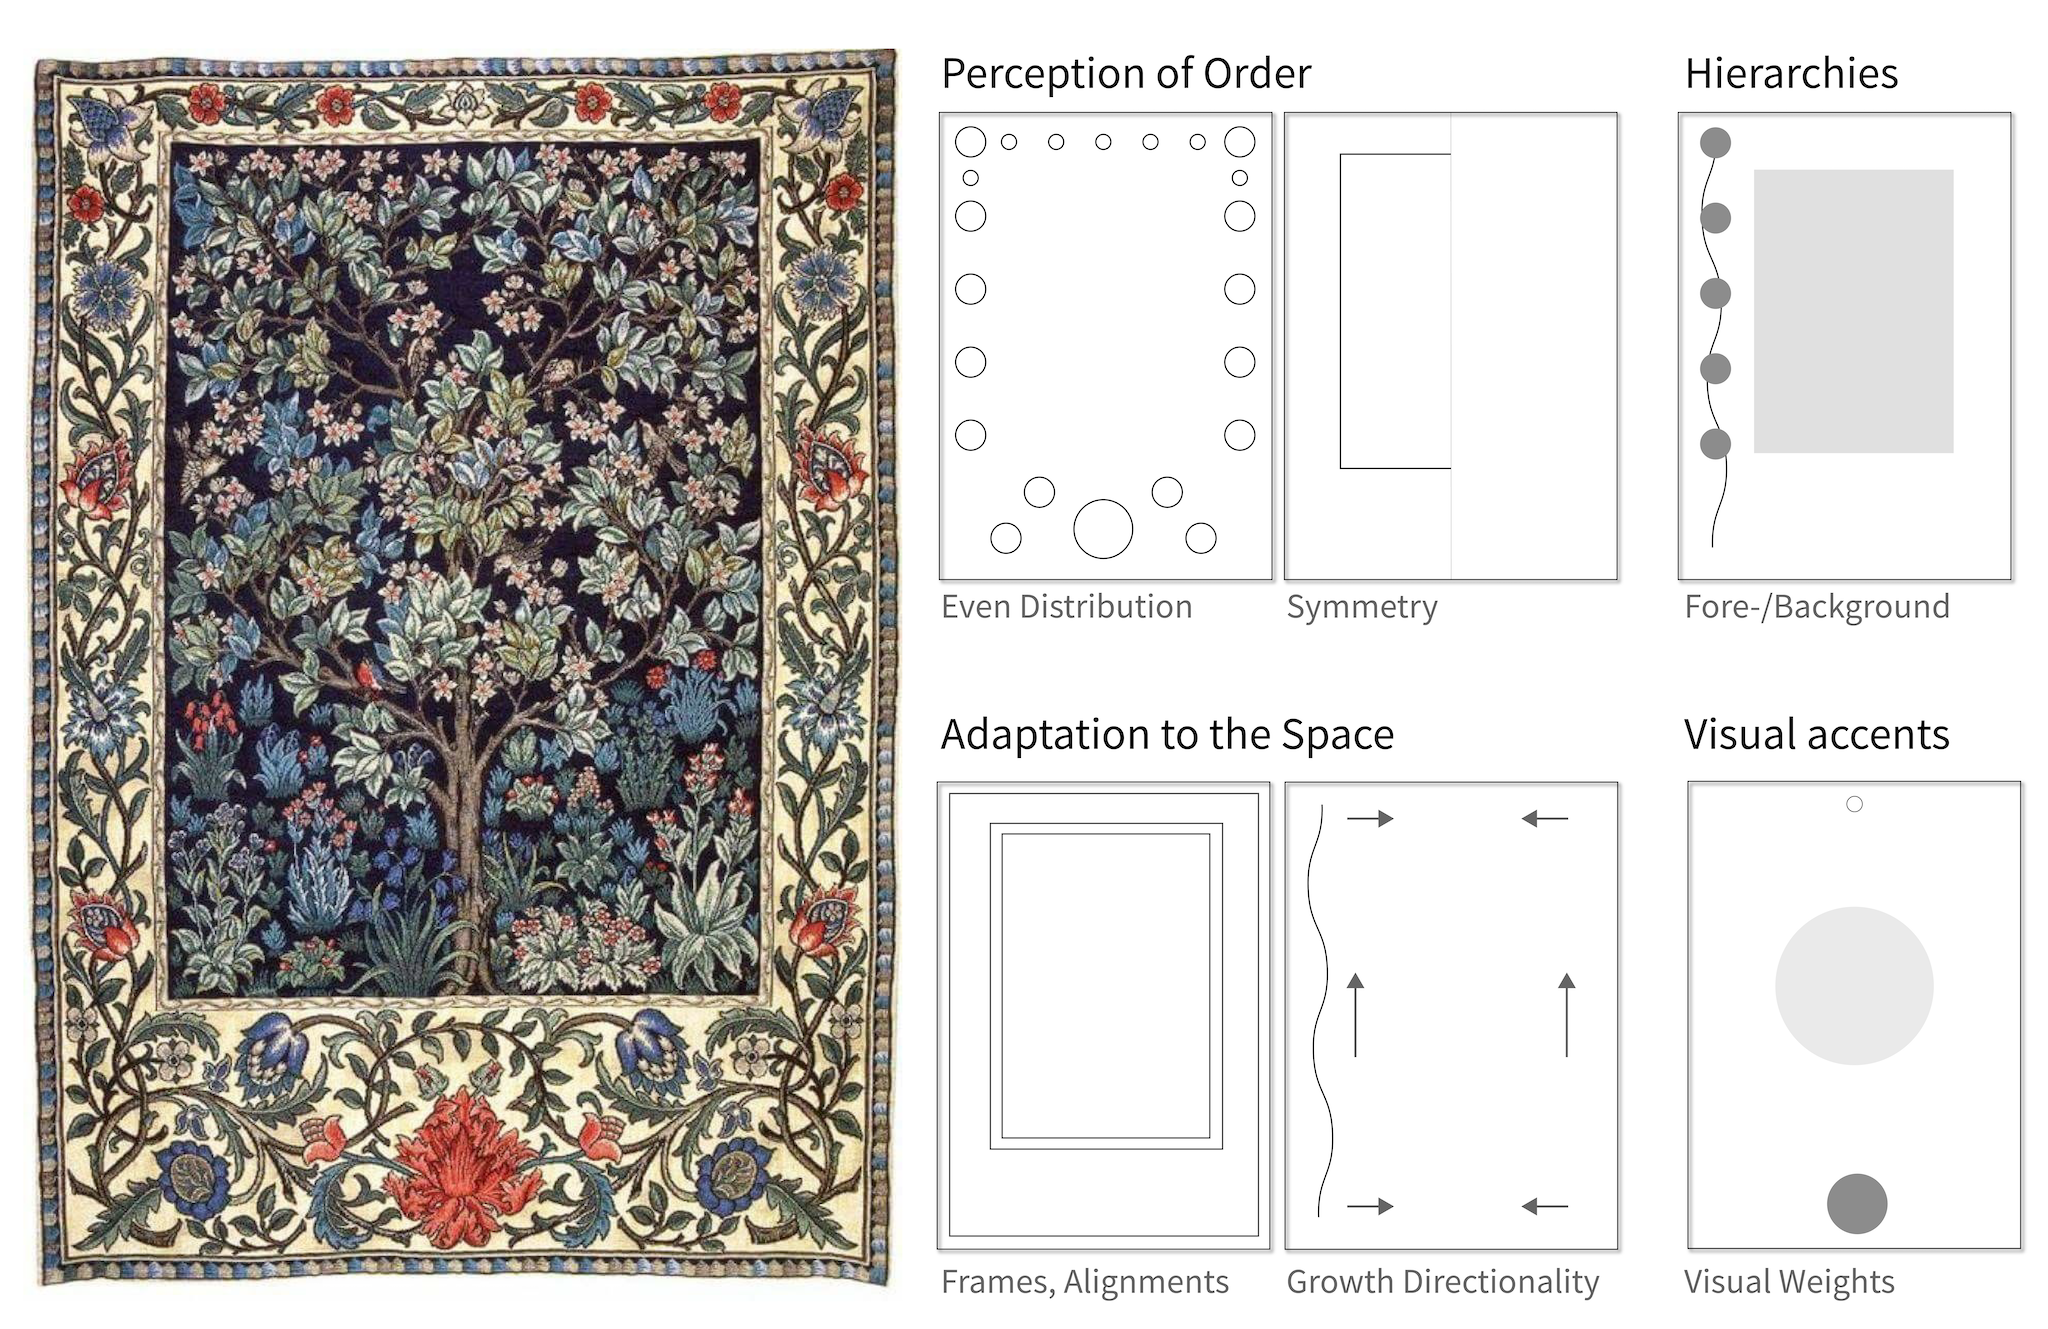
\includegraphics[width=1\columnwidth]{figures/ornament/ornament_principles.png}
%  \caption[Ornamentation principles]{\label{fig:ornamentation_principles} Exemplary dissection of visual characteristics fulfilling ornamental principles. Single features often support several principles, as, for example, the frames and borders create a hierarchical composition, an adaption to the space the ornament fills and visual contrasts. Image source left image: [11]}
% \end{figure}

% \subsection{Summary}
% \label{subsec:design_summary}

% Creative pattern generation differentiates itself from homogeneous pattern creation by including aspects such as distribution and repetition, curves, lines and sketches, frames and hierarchies, connections, branches and directionality, and single accents. Creative pattern generation exemplifies the common challenge of enabling control for tasks for which humans are indispensable in combination with the automation of tedious manufacturing and the computation of structuring rules. With that it is a representative design goal to aspire to for a general investigation of creative control mechanisms.
